\chapter*{Preface} % (fold)
\label{cha:preface}
This thesis is divided into two parts. The first part covers work done at the Muon Science Innovative Channel (MuSIC) beam-line and the second part, discusses work carried out on the European X-ray Free Electron Laser (EuXFEL).

The first part, discussing MuSIC, has two main themes: simulation and measurement. An introduction (chapter~\ref{prt:introduction}) covers the essentials of the project and the physics behind it. Chapter~\ref{prt:simulation} describes the development of the MuSIC simulation  and its deployment in creating a rigorous analysis. Finally chapter~\ref{prt:characterising_the_beam} discusses the results of the measurements made at MuSIC.

The second part is concerned with creation of the firmware interface between the Clock and Control Card (CCC) and the Large Pixel Detector (LPD). It discusses the design, implementation and testing of the firmware ahead of use in EuXFEL.

\part{Characterisation of the MuSIC beam} % (fold)
\label{prt:characterisation_of_the_music_beam}

\chapter{Executive Summary} % (fold)
\label{cha:executive_summary}
The Muon Science Innovative Channel (MuSIC) beam line is a prototype muon production system being developed at the Research Centre for Nuclear Physics (RCNP) in Osaka, Japan. It uses a novel Pion Capture Solenoid (PCS) that captures a much larger fraction of the produced pions than other muon beam lines do. Once the pions have been captured they are directed in to the Muon Transport Solenoid (MTS) where they can decay to produce muons. MuSIC aims to achieve a muon production efficiency (per Watt of proton beam) that is far higher than is currently seen at existing beam lines. 

High flux, low power muon beams will enable the creation of dedicated muon Spin Resonance (\(\mu\)SR) devices, they are a first step in making neutrino factories as well as being vital in particle physics studies such as the measurement of rare decays (e.g.\ \(\mu\rightarrow eee\)). In addition, muon beams can be used in the development of other technologies, e.g.\ MuSIC will be used to conduct research into Fixed Field Alternating Gradient (FFAG) storage rings and test their viability as an acceleration technology for muons.

A key use of MuSIC will be as a prototype for the Coherent Muon-to-Electron Transition (COMET) experiment being built at J-PARC in Tokai, Japan. COMET will use a similar, albeit larger, pion capture solenoid to produce a pulsed beam of \(10^{11}\)~muons~s\(^{-1}\) that will enable it to make the most precise measurements of the rare muon decay: \(\mu N \rightarrow eN\). The insights gained at MuSIC, both in terms of the technology and the science, will help improve the measurements made at COMET. 

In order to better understand MuSIC it was simulated using Geant4 and G4Beamline (G4BL). Two core simulations were made, one of the PCS and MTS made using G4BL and a second of the detectors made using Geant4. The G4BL simulation was used to test the initial designs of MuSIC and later to provide realistic particle distributions for the Geant4 simulation. The detector simulation, made in Geant4, was used to test detector configurations and refine analysis techniques.

Commissioning of the PCS and the first 36\(^{\circ}\) of the MTS was completed in 2010. The final design of MuSIC has a planned 180\(^{\circ}\) MTS but the initial section is enough to begin characterising the beam. Over two years there were five periods of beam time, each lasting between 24 and 72 hours, for which the RCNP's proton beam was available for use at MuSIC. 

During the five beam times, detectors and data acquisition (DAQ) were installed, tested and used to make three different measurements that help characterise the MuSIC beam. The three measurements were of the total charged particle flux, the muon lifetime and the muon momentum spectrum. Each experiment used simple detectors made of plastic scintillators with Multi-Photon Pixel Counters (MPPC) for read out. 

The charged particle flux was measured in two separate beam times, firstly with a long strip scintillator (1\(\times\)3\(\times\)38~cm\(^3\)) and then with a disk scintillator (3.5\(\times \pi \times\)2~cm\(^3\)). The first measurement was made 6~cm from the end of the MTS at a range of heights. The peak charged particle flux was measured to be (94.3\(\pm\)4.0)\(\times10^3\)~particles~nA\(^{-1}\) at \(5\)~cm above the beam pipe's centre. The second measurement was made 85~cm from the end of the beam pipe at a range of horizontal and vertical positions. The peak flux for the second measurement was (11.16\(\pm\)0.11)\(\times10^3\)~particles~nA\(^{-1}\) at \((0, 20)\)~cm, i.e.\ directly above the beam pipe's centre. The second most intense location was at \((-17, 0)\)~cm, to the left of the beam centre (when facing it). Both these measurements show that the most intense part of the beam is above the centre and the second also shows that the this spot is slightly offset towards the left, which agrees with the simulation although not on the predicted intensity.

The muon lifetime was measured during two beam runs as a method of demonstrating the presence of muons in the beam. The measurement was made by using two scintillators on either side of a metal stopping target. By plotting the time between events in each scintillator the muon decay spectrum could be constructed and the muon's lifetime measured. The first measurement of the muon lifetime was made during the same beam time as the second charged particle measurement and recorded a lifetime of (2,016\(\pm\)89)~ns which is lower than the canonical value of (2196.9811\(\pm\)0.0022)~ns~\cite{pdg} although this is likely due to the presence of a stopping target which would have reduced the negative muon's lifetime. The second measurement attempted to account for the presence of the stopping target by fitting the muon lifetime with two exponentials and hence measured the free muon lifetime to be (2202\(\pm\)20)~ns and the lifetime of negative muons in the copper stopping target to be (195\(\pm\)17)~ns. The lifetime of muonic copper was slightly higher than the canonical value of (163.5\(\pm\)1.0)~ns measured in by Suzuki~et~al.~\cite{suzuki_mu_capture_rates} but is still in reasonable agreement.

The final measurement, the muon momentum spectrum, was the most complex. Six measurements were made using one of four different thickness aluminium degraders. The degraders reduced the energy of any charged particles and so filtered out different momentums to stop on the copper stopping target. By plotting the decay spectrum and integrating the area under the exponential portion it was then possible to count the number of stopped muons and hence estimate the number of muons of that momentum. The momentum spectrum measured for freely decaying muons is shown in figure~\ref{fig:exec_summary_muon_momentum_spectrum}. This figure also shows the reasonable agreement between the simulation and the measurement although the errors on the measurement are large. 

\begin{figure}[htpb]
  \centering
    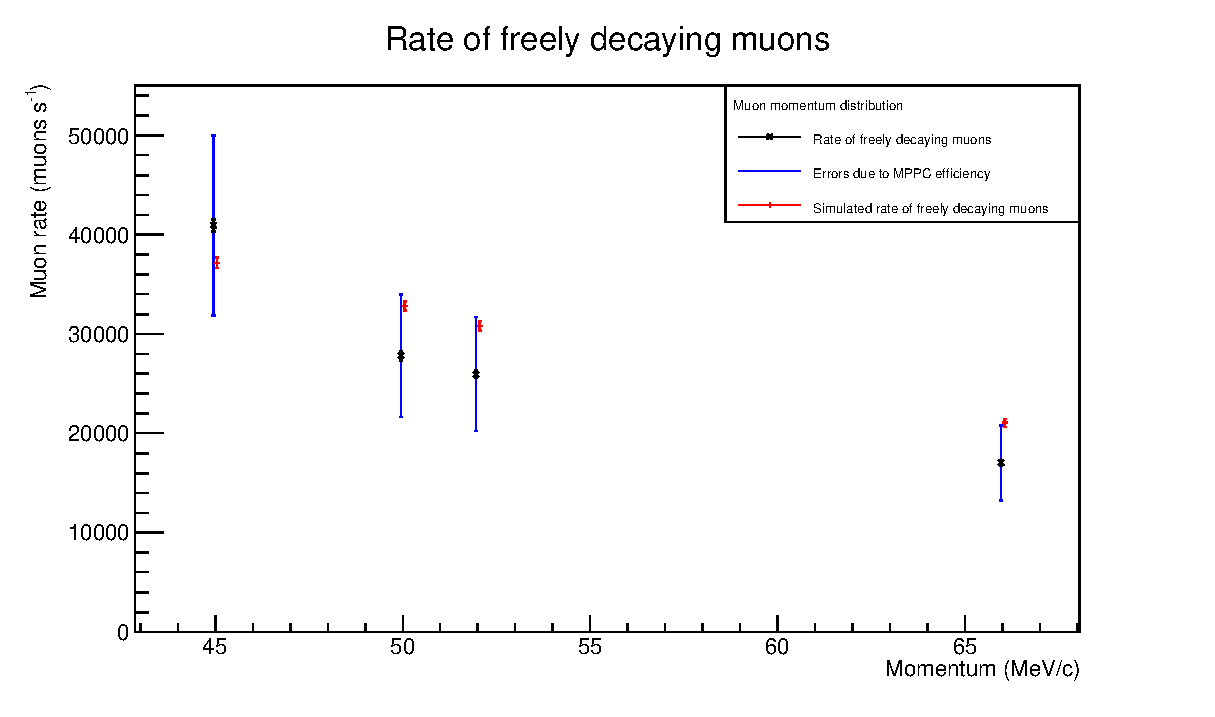
\includegraphics[width=.9\textwidth]{../3_measurements/images/plot_generating_scripts/adjusted_muon_rates_exec_summary_version.eps}
  \caption{Measured muon momentum spectrum for freely decaying muons at MuSIC. The muon rate is normalised to a proton beam current of 1~nA.}
  \label{fig:exec_summary_muon_momentum_spectrum}
\end{figure}

Using the data from the momentum spectrum measurement it was possible to predict the total muon flux at MuSIC when operated at full power\footnote{To prevent excessive dead time in the equipment currents of \(<\)1~nA were used rather than the RCNP's maximum current of 1~\(\mu\)A.} and this was calculated to be \((4.16\pm0.53)\times10^8\)~muons~s\(^{-1}\) which is on par with the world's most intense muon source, PSI, which has a peak flux of \(4.8\times10^8\)~muons~s\(^{-1}\). The key difference between MuSIC and PSI is that PSI produces its muons using a 1.2~MW proton beam compared to the RCNP's 400~W beam, giving per-Watt yields of \((8.3\pm1.1)\times10^5\)~muons~W\(^{-1}\) and 292~muons~W\(^{-1}\) respectively therefore MuSIC is the most efficient muon source in the world.

% chapter preface (end)
%%%%%%%%%%%%%%%%%%%%%%%%%%%%%%%%%%%%%%%%%%%%%%%%%%%
\chapter{Introduction} % (fold)
\label{prt:introduction}
MuSIC is a new muon source housed at the Research Centre for Nuclear Physics (RCNP) in Osaka, Japan. Commissioning of the beam began in 2010 with installation of the Pion Capture System (PCS) and the first 36\(^{\circ}\), of a planned 180\(^{\circ}\), of Muon Transport Solenoid (MTS). To date there have been five periods of beam time.

Over the course of the five sessions of beam time three core measurements have been made that will be discussed in this thesis:
\begin{enumerate}
  \item Charged particle flux.
  \item Muon lifetime.
  \item Muon momentum spectrum.
\end{enumerate}
All of these experiments have had the aim of characterising the beam at MuSIC and confirming the efficiency of muon production. The measurements themselves are discussed in chapter~\ref{prt:characterising_the_beam}.

While still incomplete, enough of MuSIC exists to test the efficacy of the PCS and existing MTS. The PCS uses a novel design in order to to maximise muon production. This new design is predicted to be several orders of magnitude more efficient than current methods.

The rest of this chapter is divide into three sections: Muon sources (section~\ref{cha:high_intensity_muon_sources}), MuSIC (section~\ref{cha:music}) and physics (section~\ref{cha:physics}). `Muon sources' discusses existing muon beams and goes on to make the case for high intensity muon sources. The section on MuSIC discusses its design and the scientific motivation for building it. Finally the physics section reviews the theory behind charged particle interactions in matter, muon decay and charged Lepton Flavour Violation (cLFV).

\section{Muon Sources} % (fold)
\label{cha:high_intensity_muon_sources}
The muon was the first second-generation particle to be discovered, it has been used to test the theory of relativity~\cite{rossi_hall_first_muons}, measure the size of the proton~\cite{proton_size} and to measure oscillations of neutrinos~\cite{t2k_cdr}. Not only is the muon an interesting particle in its own right, but a powerful and precise tool of further research. 

Muons are a lepton; they are \(\sim\)200 times more massive than their sibling, the electron\footnote{The mass of the muon is 105.6583715\(\pm\)0.0000035~MeV, an electron is \( 510.998928\pm0.000011 \)~keV~\cite{pdg}.}. Unlike the electron, muons can decay and the majority of the time\footnote{\(\approx100\%\) of the time~\cite{pdg}.} muons decay via the process \(\mu\rightarrow e\nu\overline{\nu}\), the muon's lifetime prior to undergoing decay is 2.1969811\( \pm \)0.0000022~\( \mu \)s~\cite{pdg}. Muons interact via the electroweak forces and are, as far as we know, elementary particles.

More than any other property, the lifetime of the muon, encompass the biggest problem with muon sources. The fact that muons decay; unlike protons, neutrons\footnote{The neutron's lifetime is \(880.0\pm0.9\)~s~\cite{pdg} long enough to make it stable in comparison to the muon.} and electrons, makes manipulating muons a race against time. All beams have similar stages: production, acceleration, cleaning and finally deployment; for muons this has to happen in the 2.2~\(\mu\)s that the muons exist for. Despite the difficulty of creating muon beams the usefulness of a non-electron lepton beam is not to be underestimated.

As a particle that isn't common in nature muons cannot be produced in the same way as, e.g.\ electrons: via ionisation and subsequent acceleration. The most common method for muon production is via pion decay (see figure~\ref{fig:pion_decay_feyman}), this process has a branching ratio of 99.98770$\pm$0.00004~\%~\cite{pdg}\footnote{The next most common decays are \( \pi\rightarrow\mu\nu_{\mu}\gamma \) and \( \pi\rightarrow e \nu_e \) which have branching ratios of \( (2.00\pm0.25)\times10^{-4} \)\% and \( (1.230\pm0.004)\times10^{-4} \)\% respectively.}. The pion has a lifetime of only 26.033\(\pm\)0.005~ns~\cite{pdg}, i.e.\ \( \sim \)1\% of the lifetime of the muon meaning that given a suitable amount of time, the pion contamination of the muon beam can be kept low. Pion production occurs through proton-proton interactions above the energy threshold of \( \sim380 \)~MeV. The simplest method achieving proton-proton interactions above the pion production threshold is through the bombardment of a fixed target with a proton beam.

\begin{figure}[hptb]
  \centering  
    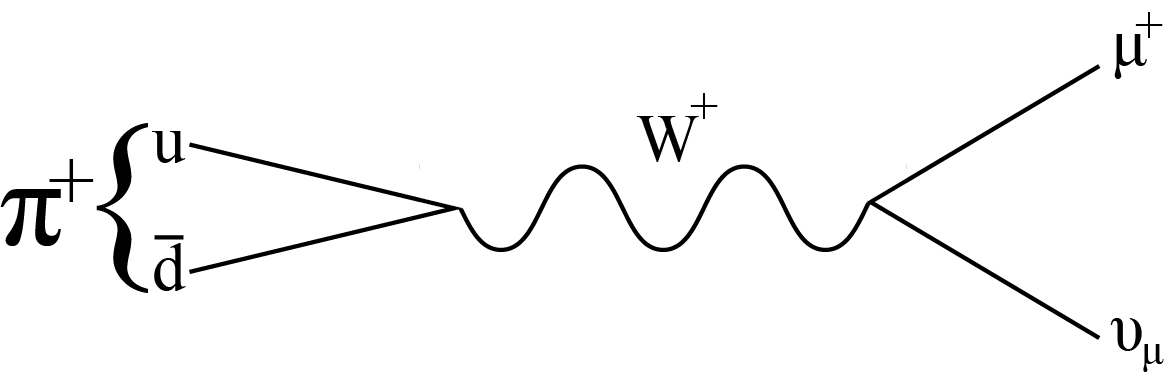
\includegraphics[scale=0.8]{images/pion_decay_feyman.png}
  \caption{Feynman diagram showing muon production through pion decay.}
  \label{fig:pion_decay_feyman}
\end{figure}

Whilst all muon sources use pion decays to generate their beams there are several broad categories of beam. Muon beams are generally categorised depending on where the muons originate: `cloud', `surface' and `sub-surface'. Most muon facilities will have one or more of each type of beam, as they are not incompatible and all have different properties. `Cloud' beams collect pions (and some muons) then transport them to a `decay pipe' in which the remainder of the pions can decay. In general cloud type beams have a larger range of momenta as the pions decay in flight. `Surface' and `sub-surface' beams are both generally of lower momenta (\( <30\)~MeV/c) than cloud types as they collect muons produced by pions decaying at rest on (or just inside) the surface of the target. Surface and sub-surface beams are in high demand for muon Spin Resonance (\(\mu\)SR, see section~\ref{sub:muon_spin_resonance}) experiments which require high fluxes of low momentum muons.

There are currently several dedicated muon sources\footnote{In theory any proton source, with energy above the pion production threshold, can operate as a muon source but only a few have dedicated facilities.} around the world (see table~\ref{tab:cf_muon_sources}). All of the current muon sources have their facilities acting in a parasitic mode on their main proton beam-line, with the majority of the proton beam being used for neutron sources. Most muon facilities have several separate beam-lines that can operate semi-independently, with each beam-line often specialising in a certain sub-set of muons. For example, RIKEN-RAL has 4 experimental ports: port-1 is used to investigate muon-catalyzed d-t fusion (\(\mu\)CF), port-2 and port-4 are dedicated \(\mu\)SR experiments; and port-3 is used for low energy muon production.

\begin{table}[htpb]
  \begin{center}
  \begin{tabular}{c | c | c | c | c | c | c}
    Name       &  \multicolumn{3}{c|}{Muon beam}                 &  \multicolumn{2}{c|}{Proton Beam}  &   Ref \\
               &  Flux (muons/s)     &  Type  & \( P \) (MeV/c)  &  Power (W)    & \(I\) (\(\mu\)A)   &       \\
    \hline    
    PSI        &  \(4.8\times10^8\)  &  Cont.  &  28  &  \(1.2\times10^6\)  &  2000  &  \cite{mue4_psi}   \\ 
    RIKEN-RAL  &  \(6\times10^5\)    &  Pulse  &  27  &  \(1.6\times10^3\)  &  200   &  \cite{riken_ral}       \\
    TRIUMF     &  \(3.5\times10^6\)  &  Pulse  &  25--85  &  \(7.0\times10^4\)  &  140   &  \cite{triumf_m20a} \\
  \end{tabular}
  \end{center}
  \caption{Comparison of several leading muon sources. As most sources have multiple muon beam-lines the highest flux station at each source was chosen: \(\mu\)E4 at PSI; port-1 of the RIKEN-RAL facility and the M20A beam-line at TRIUMF. The difference in momenta is due to both \(\mu\)E4 and port-1 using surface muons whilst M20A uses cloud muons. Beam type refers to whether the beam is continuous or pulsed. \( P \) is the muon momentum (either as an average if reasonably mono-energetic or a range), \( I \) is the proton beam's current.}
  \label{tab:cf_muon_sources}
\end{table}


\subsection{Scientific Motivation for High Intensity Muon Sources} % (fold)
\label{sec:scientific_motivation_for_high_intenstity_muon_sources}
As has been noted muons are highly active area of research, both as a tool for further research and a focus of study. The activity surrounding muon beams is only increasing as new technologies become available and our ability to control these short lived beams increases. 

As a focus for study, in and of themselves, muons present several interesting avenues for research. Muons are a well understood particle whose interactions are known to high precision. Because muons are so well understood they make an excellent arena to test the limits of our knowledge: by making precision measurements of the muon and its interactions we can test regions of theory that are otherwise inaccessible. For example, by looking for charged Lepton Flavour Violating (cLFV, see section~\ref{sec:charged_lepton_flavour_violation}). Through cLFV processes such as \( \mu\rightarrow eee \) or \( \mu N \rightarrow N^* e \), we can test the limits on many `beyond the Standard Model' theories. Obviously, in order to measure a process that has, so far, never been seen you need an ample supply of the source material so high intensity muon sources are vital for these measurements.

Currently one of the most active areas of research in particle physics is that of neutrinos. Whilst very common in nature the neutrino's tiny cross section makes study of it very difficult. In recent years this has been solved through the creation of neutrino beams such as T2K~\cite{t2k_cdr}. Neutrino beams are normally created using the decay products of pions but there is growing interest in building so-called `neutrino factories'. One proposed design for a neutrino factory uses an oval storage ring to hold muons until they decay to create a mixed electron/muon-neutrino beam, obviously if many more neutrinos are wanted then then significantly higher intensity muon sources are needed.

A commonly described evolution of the neutrino beam is to create a second muon beam and counter rotate them in order to produce a muon collider. A leptonic collider is highly attractive: as elementary particle collisions are cleaner and can be more finely controlled whilst the higher mass of the muon over the electron means that there is much less energy loss to synchrotron radiation. A muon collider would present many challenges but with the International Linear Collider (which uses electrons) expected to be \(\sim\)31~km long~\cite{ilc} smaller, more complex, colliders become alternative options. If a muon collider can be built as the next stage of a neutrino factory, so much the better.

Particle physics presents just one facet of the many uses to which muon beams can be put. One of the most common uses of muon beams is probing the magnetic properties of materials through \(\mu\)SR, other applications include using muons to determine the nuclear matrix elements of materials, measuring trace elements in a sample through the emission of muonic X-rays and research into \(\mu\)CF.

% section scientific_motivation (end)
%%%%%%%%%%%%%%%%%%%%%%%%%%%%%%%%%%%%%%%%%%%%%%%%%%%
% chapter high_intensity_muon_sources (end)
%%%%%%%%%%%%%%%%%%%%%%%%%%%%%%%%%%%%%%%%%%%%%%%%%%%
\section{MuSIC} % (fold)
\label{cha:music}
% TODO Introduction: MuSIC Obligatory pictures of final design of MuSIC & current status
MuSIC is a proof of concept beam-line that aims to produce the most muons per proton of any existing source. MuSIC aims to have a muon flux comparable to that of PSI's (the current world best) using a beam with \(^1/_{3,000}\) the power. This can be done by one of two naive methods: increasing the efficiency of production or using a more powerful initial beam. At both RIKEN-RAL and PSI the muon beams are produced using only a fraction of the initial proton beam. It is common that less than 10\% of the initial proton beam is used to create muons, the rest continues to neutron sources. Obviously to create a high intensity muon beam using as many of the protons as possible should be the first design goal. There is a second advantage to moving away from a parasitic muon production: not only is the entire proton beam used but more of the pions can be captured. In a parasitic design the PCS has to allow the for the continuation of the proton beam, this places limits on the geometry that can be used and produced sub-optimal efficiencies. If the requirements for a continuing proton beam are removed though, the PCS geometry can be optimised purely for pion capture making further gains over merely increasing the proton current.

\begin{figure}[htbp]
  \centering
    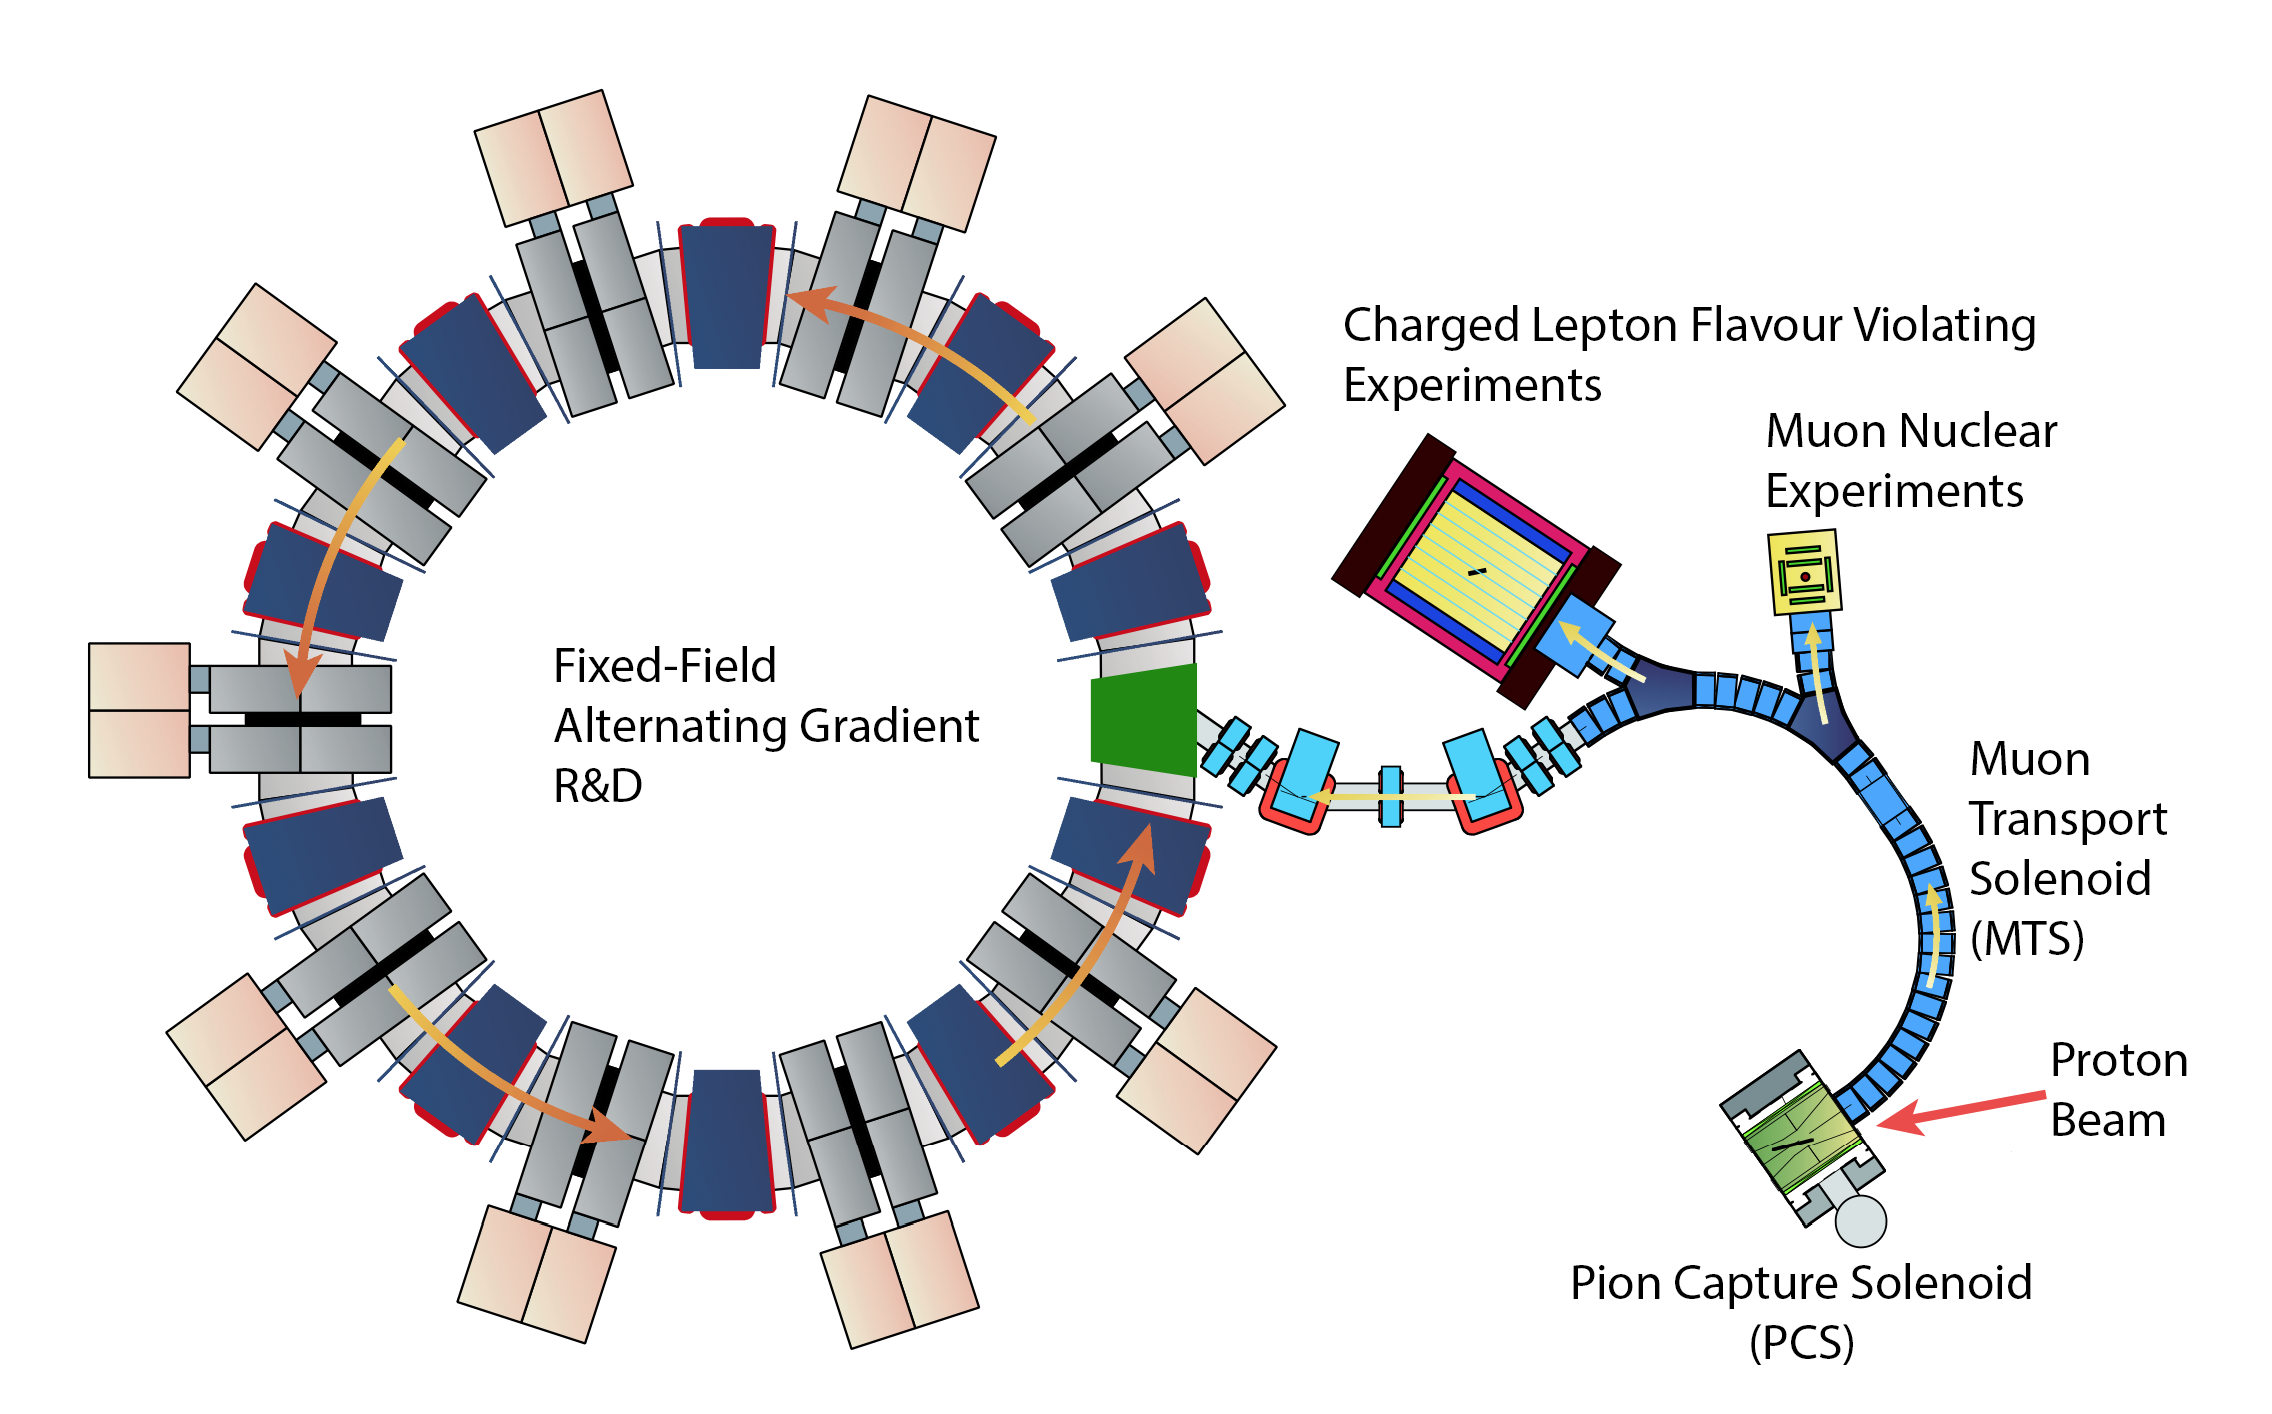
\includegraphics[width=.9\textwidth]{images/MuSIC_schematic_FFAG.png}
  \caption{Schematic of the completed MuSIC complex.}
  \label{fig:images_MuSIC_schematic_FFAG}
\end{figure}

\begin{figure}[htbp]
  \centering
    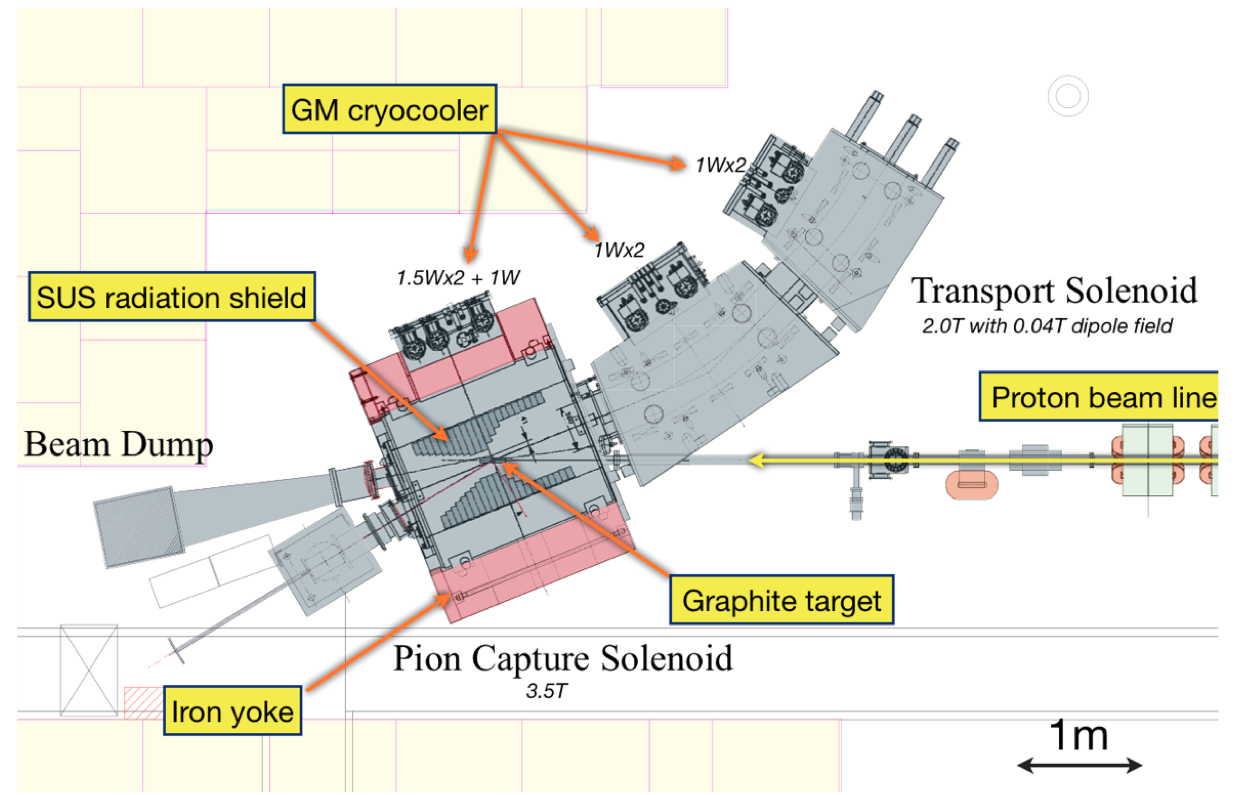
\includegraphics[width=.9\textwidth]{images/MuSIC_current_schematic.png}
  \caption{Schematic of the current status of MuSIC.}
  \label{fig:images_MuSIC_current_schematic}
\end{figure}
\begin{figure}[htbp]
  \centering
    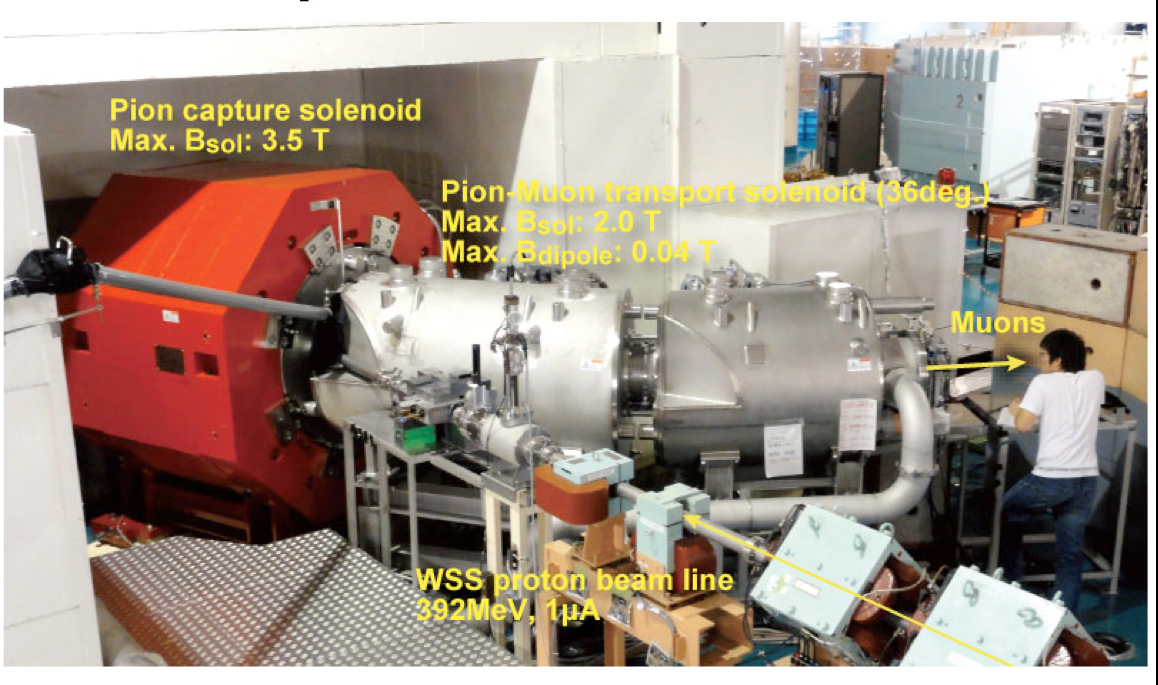
\includegraphics[width=.9\textwidth]{images/MuSIC_photo.png}
  \caption{Photo of MuSIC showing its 2010 status, since then it has had further concrete blocks added around it to increase shielding.}
  \label{fig:images_MuSIC_photo}
\end{figure}

Figure~\ref{fig:images_MuSIC_schematic_FFAG} shows the expected complete MuSIC complex including the proposed experimental stations. The schematic in figure~\ref{fig:images_MuSIC_current_schematic} shows the current status, with the Pion Capture System (PCS) and the first 36\(^{\circ}\) of Muon Transport Solenoid (MTS) complete. Figure~\ref{fig:images_MuSIC_photo} is a photo of the status of MuSIC in 2010, prior to the addition of further shielding.

\subsection{MuSIC design} % (fold)
\label{sec:music_design}
The core component of MuSIC is its PCS. The MuSIC PCS is designed to use as much of the proton beam and capture as many pions as possible. The PCS achieves this with a \(2.1\times2.4\times1.6\)~m\(^3\) super-conducting magnet that has a maximum strength of 3.5~T. The PCS has an extremely large solid angle making MuSIC capable of capturing a significant portion of the pions and directing them into the muon transport solenoid (MTS).

The MTS is intended to perform three roles within MuSIC: the collection and decay of travelling pions; selection of low-energy (30--50~MeV) muons and selection of muon charge. Ultimately the MTS will form a 180\(^{\circ}\) semi-circle but currently only the first 36\(^{\circ}\) has been constructed. The MTS's designed 10~m length provides the requirements for pion decay; its radius and magnetic field provide momentum selection whilst the application of a dipole field will select charge. Like the PCS the MTS uses super-conducting magnets to provide the 2~T main field and the 0.04~T dipole field.

The proton beam for MuSIC is provided by the RCNP's ring cyclotron. The cyclotron produces a 400~MeV proton beam (enough for pion production) with a maximum current of 1~\(\mu\)A giving a maximum power of 400~W. The beam is produced in an ion source then accelerated using two cyclotrons: the AVF and then the ring cyclotron. The first cyclotron, AVF, can accelerate a variety of ions (up to \(^{18}\)O) using a voltage of 60~kV, for protons this corresponds to a final energy of \(\sim\)65~MeV. The ring cyclotron then accelerates the protons to \( \sim \)400~MeV. 

The MuSIC PCS has been optimised to capture backwards travelling pions and muons with a maximum transverse momentum (\(P_{T}^{max}\)) of 52.5~MeV. The two key parameters that determine \(P_{T}^{max}\) are the magnet's bore and the field strength, through optimisation these were determined to have values 10~cm and 3.5~T respectively. To obtain a 3.5~T field copper-stabilized NbTi superconductor was used, this requires cooling to 4~K which is achieved through the use of 3~GM cryocoolers. 

The target used is a graphite cylinder 20~cm long with a 2~cm radius. To maximise production the target is rotated from the PCS axis to align its major axis with the proton beam. The superconducting magnet is shielded using stainless steel that has a maximum thickness of 27~cm, the shielding tapers on either side of the target (see figure~\ref{fig:images_MuSIC_current_schematic}). The taper is more rapid in the backwards direction in order to capture the maximum number of pions and muons.  

As already noted the muon transport solenoid (MTS) has to select muon momentum and charge whilst letting pions decay. The MTS has a designed length of 10~m which is predicted to reduce the pion contamination to less than 0.1\%. Application of the dipole field can be used to select charge.

% section music_design (end)
%%%%%%%%%%%%%%%%%%%%%%%%%%%%%%%%%%%%%%%%%%%%%%%%%%%
\subsection{MuSIC: Scientific Motivation} % (fold)
\label{sec:music_scientific_motivation}
The general arguments for high intensity muons beams have already been presented (section~\ref{sec:scientific_motivation_for_high_intenstity_muon_sources}), MuSIC, though is not technically a high intensity muon beam. Assuming that it meets full design specifications it should have a comparable intensity to the muon beam-lines at PSI. To this end the scientific case for MuSIC is slightly different to that for a full high intensity muon beam. The key aim of MuSIC is in proving the PCS and MTS technology, what PSI achieves with a 1.3~MW proton beam MuSIC aims to achieve with a 400~W beam. This section will set out the other uses to which MuSIC will be put.

\subsubsection{Prototype for COMET} % (fold)
\label{sub:prototype_for_comet}
The COherent Muon to Electron Transition (COMET~\cite{comet_cdr}) experiment intends to place the most stringent limits in the world on the charged Lepton Flavour Violating (cLFV) decay \( \mu + X \rightarrow e + X \). According to the Standard Model, including neutrino oscillation, this decay should have a branching ratio of \( \sim 10^{-54} \) which is far beyond current detector capabilities, this means that should such a decay be seen it would be a the so-called `smoking gun' of new physics. Many beyond the Standard Model theories (e.g.\ \cite{clfv_in_susy}) predict this decay at branching ratios that should be detectable (\(\sim 10^{-16}\)). The design of COMET calls for a pulsed muon rate of \( \sim 10^8 \)~muons/s. In order to achieve this a PCS similar to that of MuSIC is required but with a larger field (5~T) in order to cope with the more powerful muon beam. A MTS similar to that of MuSIC's is also planned in order to select low momentum muons that can be stopped on titanium target.

The first goal of the measurements made at MuSIC is to verify that the intensities required for COMET are feasible, they will be used to refine the simulations used at COMET allowing a more well optimised final design. Additionally the expertise and techniques developed at MuSIC should be directly applicable to aspects of COMET's running, for example in gauging expected secondary particle fluxes.

% subsection prototype_for_comet (end)
%%%%%%%%%%%%%%%%%%%%%%%%%%%%%%%%%%%%%%%%%%%%%%%%%%%
\subsubsection{Precision Measurements of cLFV muon decays} % (fold)
\label{sub:precision_measurements_of_clfv_muon_decays}
As well as supporting COMET's search for \( \mu + X \rightarrow e + X \) it is planned that MuSIC will run a complementary search for the cLFV decay \( \mu \rightarrow eee \)~\cite{music_cdr}. Whereas COMET's main background is beam related and mitigated through the use of a pulsed beam, the main background to \( \mu \rightarrow eee \) at MuSIC is expected to be accidental, meaning that a continuous beam poses fewer additional problems and the benefit of a higher rate.

Using a novel detector design MuSIC aims to improve on the current limit of \( 1.0\times10^{-12} \), set in 1988 by the SINDRUM I collaboration~\cite{sindrum_1_mu_eee}, by a factor of \( \sim150 \). Exclusion at this level would limit beyond Standard Model physics to an effective mass scale of \( \mathcal{O}\)(1,000)~TeV (see section~\ref{sec:charged_lepton_flavour_violation}).

This improvement will be achieved through a higher stopping rate, longer running time and increased acceptance. Obviously a more intense, longer, run will increase the number of accidentals by a predicted factor of 2,000. To compensate for the increased background, improvements to the timing, vertex, energy and momentum detection will be needed but it is envisaged that these are attainable.

As discussed in section~\ref{sub:prototype_for_comet} detection of a cLFV event would be a huge discovery and by searching for such processes both at COMET and MuSIC a far greater region of phase space can be excluded. 

% subsection precision_measurements_of_clfv_muon_decays (end)
%%%%%%%%%%%%%%%%%%%%%%%%%%%%%%%%%%%%%%%%%%%%%%%%%%%
\subsubsection{Muon Spin Resonance} % (fold)
\label{sub:muon_spin_resonance}
Muon Spin Resonance (\( \mu \)SR) is a technique in which a highly polarised beam of low-energy (\( <50 \)~MeV) muons are used to detect the internal magnetic structure of a sample. The muons are stopped on the surface to be studied and the resultant positron recorded. By studying the distribution of the emitted positrons it is possible to determine the magnetic structure of the material. 

\( \mu \)SR is an obviously powerful technique in determining the properties of a material and is becoming increasingly useful as the study of super-conductors increases. Used in concert with the existing, pulsed, \( \mu \)SR facilities at J-PARC, MuSIC would provide a powerful tool for investigating a wide range of materials.

% subsection muon_spin_resonance (end)
%%%%%%%%%%%%%%%%%%%%%%%%%%%%%%%%%%%%%%%%%%%%%%%%%%%
\subsubsection{Fixed-Field Alternating Gradient research} % (fold)
\label{sub:ffag_research}
% TODO:Introduction : FFAG research: ref me
One of the biggest obstacles to the development of a muon-collider is the acceleration of the beam. In a traditional electron accelerator a large synchrotron ring can be used to store and accelerate a beam over a long time period, unfortunately, with their short lifetime this technique is not viable for muons. One proposed solution to this problem is to use a Fixed Field Alternating Gradient (FFAG) storage ring. An FFAG uses a fixed magnetic field that has a non-uniform gradient to accelerate and store a beam.

FFAGs are considered as a potential storage ring for muons as they can rapidly accelerate a particle without adjustment of the magnets. In this way many designs for muon colliders plan to use FFAGs to accelerate a collimated (`cooled') muon beam prior to collision. The RCNP facility already hosts a six-segment FFAG that has been used to explore phase-rotation of an alpha-particle beam. Once MuSIC is completed it is intended that these phase-rotation and further acceleration experiments be carried out on a muon beam.
% subsection ffag_research (end)
%%%%%%%%%%%%%%%%%%%%%%%%%%%%%%%%%%%%%%%%%%%%%%%%%%%
% section music_scientific_motivation (end)
%%%%%%%%%%%%%%%%%%%%%%%%%%%%%%%%%%%%%%%%%%%%%%%%%%%
% chapter music (end)
%%%%%%%%%%%%%%%%%%%%%%%%%%%%%%%%%%%%%%%%%%%%%%%%%%%
\section{Physics} % (fold)
\label{cha:physics}
This chapter covers the two primary physics processes of concern in characterising the beam at MuSIC: particle interactions with matter and muon decays. There is also a brief discussion of cLFV which is one of the main scientific motivations for MuSIC. 
\subsection{Charged Particle Interactions in Matter} % (fold)
\label{sec:charged_particle_interactions_in_matter}
All charged particles will ionise matter they pass through, the amount that any particular particle ionises any particular material is highly complex and beyond the scope of this discussion, a more thorough discussion can be found in many reviews (e.g.\ ~\cite{pdg}). The general properties of ionisation are described by the Bethe formula:
\begin{equation}\label{eq:bethe_formaula}
  -\left\langle\frac{dE}{dx}\right\rangle = Kz^2\frac{Z}{A} \frac{1}{\beta^2}\left[\frac{1}{2}\ln\frac{2m_{e}c^{2}\beta^2\gamma^2T_{max}}{I^2} -\beta^2 - \frac{\delta(\beta\gamma)}{2}\right]
\end{equation}
Where:
\begin{itemize}
  \item \( -\left\langle\frac{dE}{dx}\right\rangle \) is the average energy loss in MeVg\(^{-1}\)cm\(^2\)
  \item \( K = 4\pi N_A r^2_e m_e c^2\), (\( N_A \) is Avagadro's number and \( r_e \) is the classical electron radius) 
  \item \( m_e \) the electron mass.
  \item \( c \) the speed of light.
  \item \( z \) the incident particle's charge (i.e.\ for pions and muons, 1).
  \item \( Z \) the atomic number of the target atom.
  \item \( A \) the atomic mass.
  \item \( \beta \) is the incident particle's speed as a fraction of \( c \) (i.e.\ \( \frac{v}{c} \)).
  \item \( \gamma \) is the particle's gamma factor (i.e.\ \( \frac{1}{\sqrt{1-\beta^2}} \)).
  \item \( T_{max} \) is the maximum energy that can be transferred to a free electron in a single collision with the incident particle.
  \item \( I \) is the mean excitation energy (in eV).
  \item \( \delta(\beta\gamma) \) is the correction to the energy loss due to the `density effect'
\end{itemize}
The Bethe formula is generally applicable to any charged particle but the values for the density effect and mean excitation are not: their values are different for electrons when compared to heavier particles (e.g.\ muons and pions). Another important note is that, for electrons at low energies, whilst ionisation is the dominant effect there are other processes that need to be taken into consideration (Bhabha scattering, \(e^+\) annihilation, M\o ller scattering). 

As momentum is increased another difference between electrons and other particles appears, at higher energies electron energy loss is dominated by Bremmstrahlung whilst muons and pions' energy loss is dominated by radiative losses, this difference can be seen in figures~\ref{fig:mu-pi-bethe} and~\ref{fig:electron_energy_loss} for muons and electrons respectively. As can be seen for electrons there is no plateau between ionisation and Bremmstrahlung regime, as there is for muons for pions.  
\begin{figure}[hptb] 
  \centering
    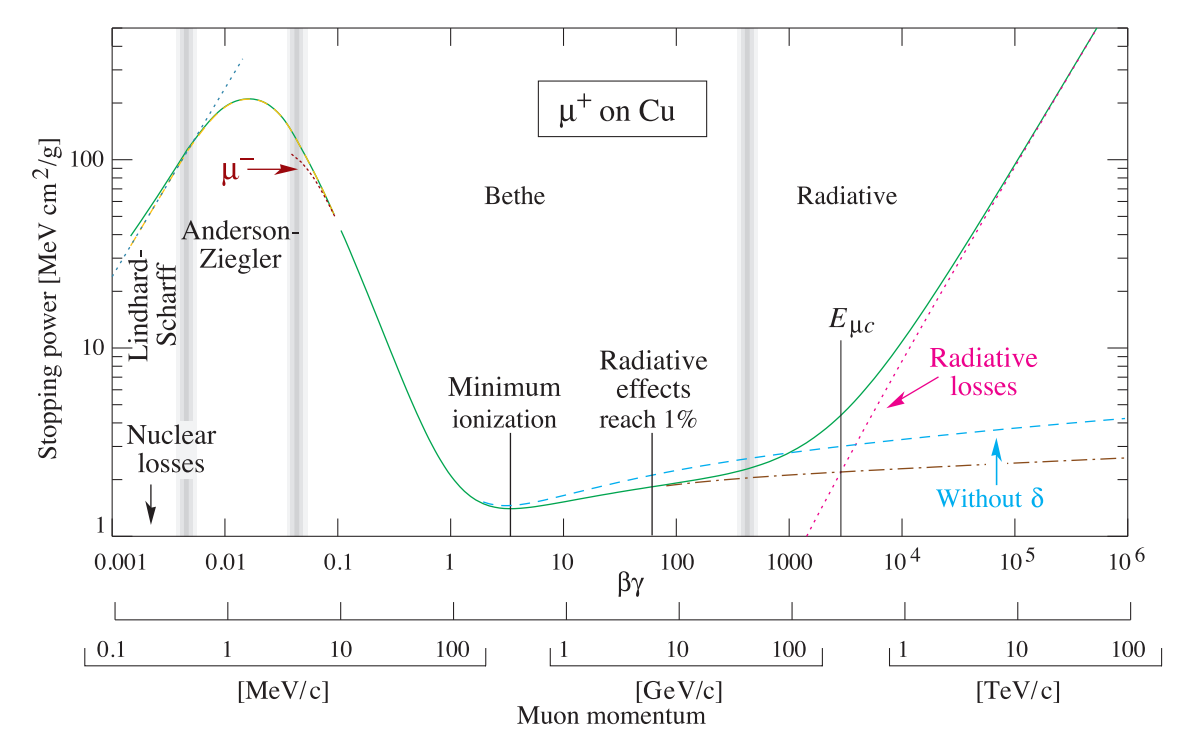
\includegraphics[width=.9\textwidth]{images/mu-pi-bethe.png}
  \caption{Energy loss by a muon in copper as a function of \( \beta\gamma \) or momentum. The solid line indicates the total stopping power, dashed lines indicate different contributions and the vertical grey bands indicate the different phenomenological regimes. Taken from ref~\cite{pdg}.}
  \label{fig:mu-pi-bethe}
\end{figure}
\begin{figure}[hptb]
  \centering  
    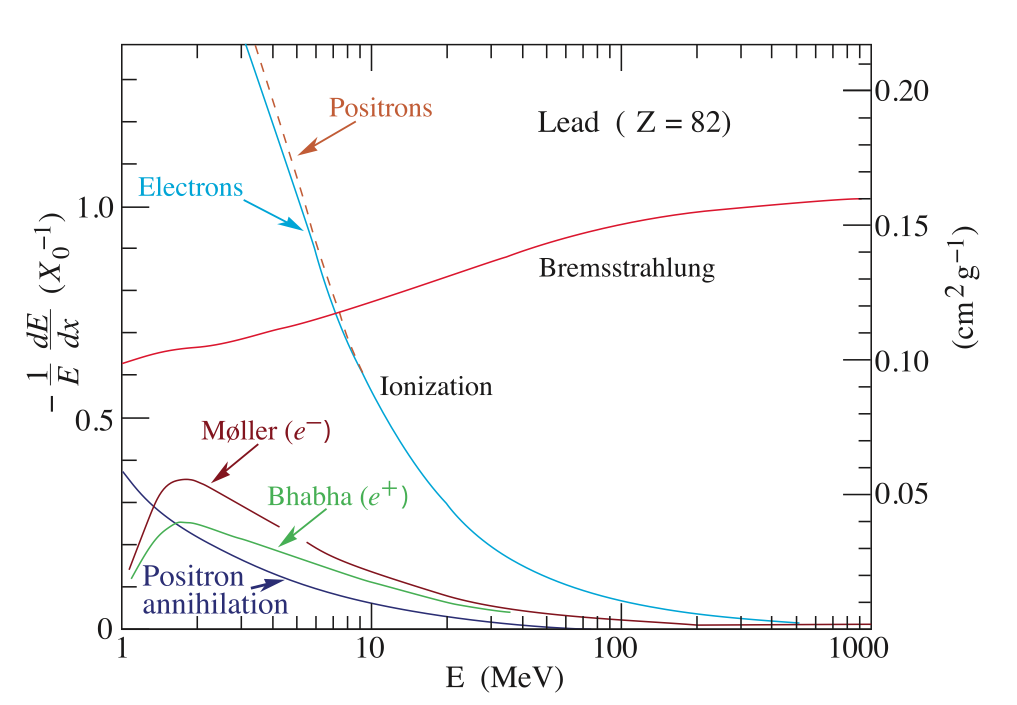
\includegraphics[width=.9\textwidth]{images/electron_energy_loss.png}
  \caption{Electron energy loss per `radiation length' (\( X_0^{-1} \)) as a function of electron energy (not momentum). The material in this case is lead (\(Z=82\) and \(X_0 = 6.37\)g/cm\(^2\)). Taken from ref~\cite{pdg}.}
  \label{fig:electron_energy_loss}
\end{figure}

At MuSIC the loss of energy by charged particles to matter is very important as it is the main method for detecting particles, and hence, characterising, the beam. When a particle deposits energy in certain materials they will produce light, this light can then be detected giving information on the beam. The exact amount of light produced is dependent on the material and the amount of energy deposited but for many materials it can be approximated to a linear function of energy deposited. There are obviously problems with assuming linear light yields but a larger problem is the non-linear function for energy deposition. 

% section charged_particle_interactions_in_matter (end)
%%%%%%%%%%%%%%%%%%%%%%%%%%%%%%%%%%%%%%%%%%%%%%%%%
\subsection{Muon decay} % (fold)
\label{sec:muon_decay}
As has been noted muons decay \(\approx100\)\% of the time through the process: \( \mu \rightarrow e \nu \overline{\nu}  \). This process is the same for both positive and negative muons, although there is a sign change and the neutrino/anti-neutrino flavours will swap. The biggest difference between positive and negative muons is that negative muons can become bound to a nucleus in the same way as electrons. This section will start with a general discussion of the important parameters of muon decay and then continue with a discussion of how this property of negative muons changes their decay.

The decay of a muon, like any other decay, can be modelled using the distribution:
\begin{equation}\label{eq:poisson}
  P(t) = Ne^{-t/\tau}
\end{equation}
Where \( P(t) \) is the survival probability of a particle after time, \( t \); \( N \) is a scaling factor to the size of the initial population and \( \tau \) is the population's lifetime. For a free muon in a vacuum the lifetime is \( \sim2.2\)~\( \mu \)s. As figure~\ref{fig:muon_decay_feynmann} shows the muon decay is mediated by a charged W boson, the presence of the two neutrinos mean that the only practically detectable result of the muon decay is the electron. The muon's (comparatively) long lifetime makes identification of them possible through by plotting decay times; this is discussed in greater detail in chapter~\ref{prt:characterising_the_beam}. 

\begin{figure}[hptb]
  \centering
    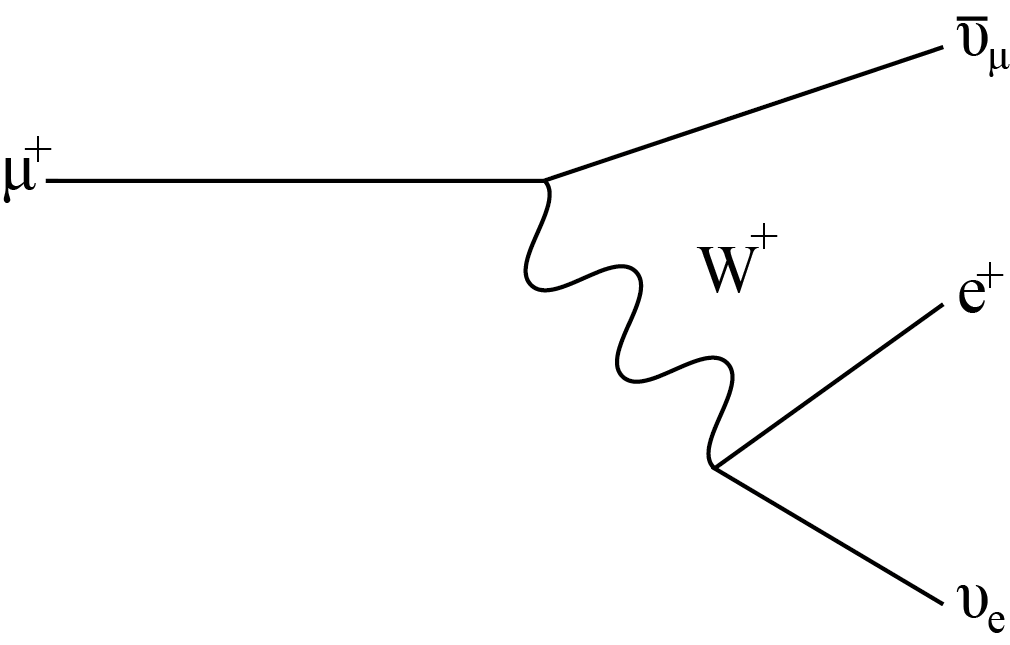
\includegraphics[scale=1]{images/muon_decay_feynmann.png}
  \caption{Feynman diagram showing muon decay.}
  \label{fig:muon_decay_feynmann}
\end{figure}

As has been noted negative muons can undergo an additional interaction with matter compared to positive muons. As a negatively charged lepton they can be become bound to a nucleus, reducing its lifetime as it loses energy falling through the nucleus' shells. The lifetime of a bound muon can be expressed as the reciprocal of an interaction rate:
\begin{align}
  \tau_{\mu^-} &= (\Delta_t)^{-1}\\
  \Delta_t &= \Delta_c + Q\Delta_d \label{eq:capture_rate}
\end{align}
where \( \Delta_t \) is the total interaction rate; \( \Delta_c \) is the rate of nuclear muon capture; \( \Delta_d \) is the rate of decay for positive muons (i.e.\ \( \tau_{\mu^+} = (\Delta_d)^{-1}  \)) modified by the `Huff-factor', \( Q \), which compensates for the reduction in energy available for a bound muon to decay. The positive, rather than negative, muon decay rate is used as the negative rate is less precisely known because of its ability to bind to a nucleus.

When a negative muon is captured by a nucleus its lifetime is reduced compared to the positive muon. This reduction is due to the muon forming a muonic atom with its captor that allows it to rapidly shed energy via X-rays as it cascades through various shells until it enters the \( 1s \) state. The muonic cascade is a very rapid event, in most materials it occurs in less than \( 10^{-13}\)s~\cite{review_nuclear_physics_mu_capture_measday}, once in the \( 1s \) state the muon will decay much sooner having lost most of its energy. As will be discussed in chapters~\ref{prt:simulation}~and~\ref{prt:characterising_the_beam} these differing lifetimes give us some insight into the ratio of positive to negative muons.

A theoretical approximation to \( \Delta_c \) as a function of atomic mass, \( A \), and atomic number, \( Z \), was devised by Primakoff and Goulard~\cite{goulard_primakoff}:
\begin{align}
  \Delta_c(A,Z)&=Z^4_{eff} G_1 \left[ 1 + G_2 \frac{A}{2Z} - G_3 \frac{A-2Z}{2Z} - G_4 \left[\frac{A-Z}{2A} + \frac{A-2Z}{8AZ} \right] \right]
  \label{eq:primakoff_and_goulard}
\end{align}
Where the values \(G_{1-4}\) are parameters to be fitted and \( Z_{eff} \) is the effective value for the atomic number, as calculated by Ford and Wells~\cite{ford_and_wills_mesonic_atoms}, which accounts for the muon's \( 1s \) radius being much smaller than an electrons. The difference between the predicted capture rate and the measured rate is given in figure~\ref{fig:primakoff-goulard_vs_exp} with the fitted values of \(G\) shown in table~\ref{tab:g1_to_g4}. As can be seen there is still a fairly large disagreement between the theory and measured values for many atoms.

\begin{figure}[hptb]
  \centering
    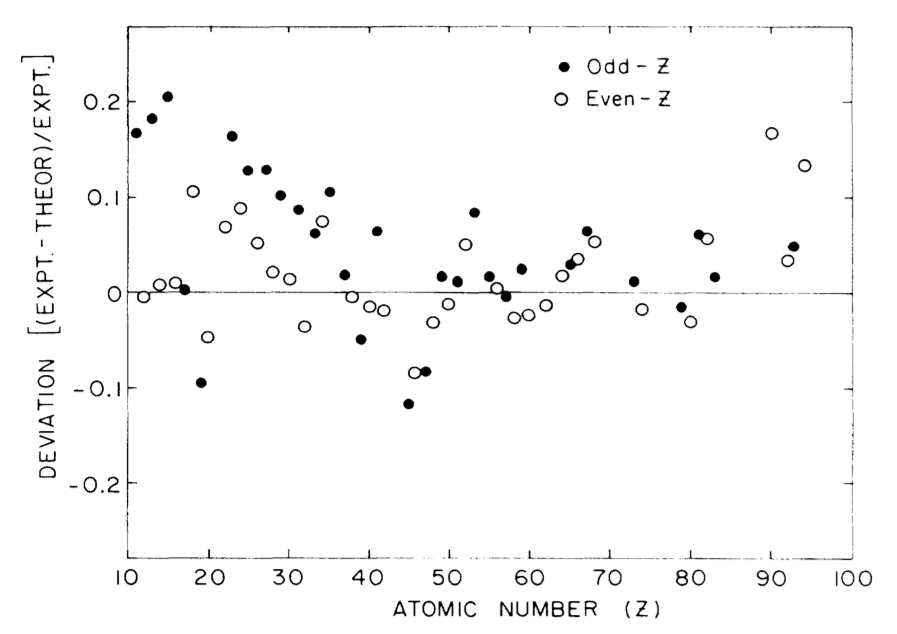
\includegraphics[width=.9\textwidth]{images/primakoff-goulard_vs_exp.png}
  \caption{Comparison of the theoretical values (as determined using the Primakoff-Goulard formula) and experimentally determined capture rates for a range of materials, taken from~\cite{suzuki_mu_capture_rates}.}
  \label{fig:primakoff-goulard_vs_exp}
\end{figure}

\begin{table}
  \begin{center}
  \begin{tabular}{c | r@{.}l }
                                                              & \multicolumn{2}{c|}{Experimental Value} \\
    \hline
    Number of data                                            & \multicolumn{2}{c|}{30}                 \\
    \hline
    \( G_1 \)                                                 &             260 &                       \\
    \( G_2 \)                                                 &              -0 & 040                   \\
    \( G_3 \)                                                 &              -0 & 26                    \\
    \( G_4 \)                                                 &               3 & 24                    \\
    \hline
    \( (\textrm{Expt.} - \textrm{Fit})/\textrm{Expt.} \) (\%) &               4 & 1                     \\
  \end{tabular}
  \end{center}
  \caption{Experimental values of \( G_1 \)--\( G_4 \) as determined by TRIUMF~\cite{suzuki_mu_capture_rates}.}
  \label{tab:g1_to_g4}
\end{table}


% section muon_decay (end)
%%%%%%%%%%%%%%%%%%%%%%%%%%%%%%%%%%%%%%%%%%%%%%%%%%%
\subsection{Charged Lepton Flavour Violation} % (fold)
\label{sec:charged_lepton_flavour_violation}
The discovery that neutrinos have mass and that they undergo flavour mixing shows that lepton flavour is not conserved, making charged Lepton Flavour Violation (cLFV) a possibility. 

In the Standard Model of particle physics the simplest diagram of cLFV is when the emitted muon neutrino is virtual (see figure~\ref{fig:images_cLFV_mu-e_conversion}), for this to be true it must undergo conversion before being absorbed by the electron; the rate of this is governed by the neutrino mixing angles and masses. In the Standard Model this processes has a very small branching ratio~\cite{effective_lagrangian_for_clfv}. E.g.\ for \( \mu\rightarrow e\gamma \), the branching ratio is: 
\begin{align}
  \text{Br}(\mu\rightarrow e\gamma) 
    &= \frac{3\alpha}{32\pi}
      \left|\sum\limits_{i=2,3} U^*_{\mu i} U_{ei}
            \frac{\Delta m^2_{i1}}{M^2_W}
     \right|^2 \\
    &< 10^{-54} \label{equ:clfv_branching_ratio}
\end{align}
where \( U_{\nu i}^{(*)} \) are elements of the neutrino mixing matrix, \(\Delta m^2_{i1}\) is difference in neutrino masses and \(M_{W}\) is the mass of the W-boson.

This extremely low branching ratio makes cLFV a `smoking gun' for new physics, should such a process be observed then it clearly indicates physics beyond the Standard Model. As a cLFV process has never been seen all current experiments have only been able to set upper limits on the branching ratio, the current world best is a limit of \(7\times10^{-13}\) set by SINDRUM~II in measuring \(\mu+Au\rightarrow e+Au\)~\cite{sindrum_2_mu_ag_e}.\footnote{This is an effective branching ratio in order to make direct comparisons with over cLFV processes easier.}

\begin{figure}[hptb]
  \centering
    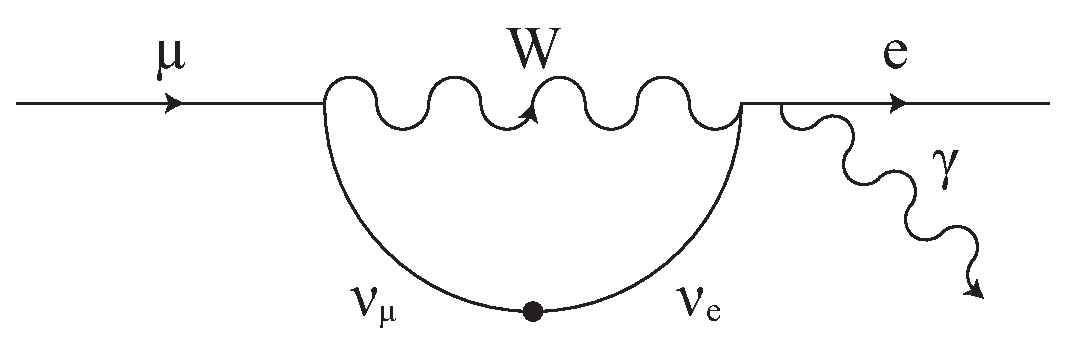
\includegraphics[width=.7\textwidth]{images/cLFV_mu-e_conversion.eps}
  \caption{\(\mu\rightarrow e\gamma\), as a Standard Model process. The black dot represents the conversion of the muon neutrino to an electron neutrino, in the Standard Model this process has a predicted branching ratio \(\sim <10^{-54} \) and has not been seen.}
  \label{fig:images_cLFV_mu-e_conversion}
\end{figure}

There are three core cLFV processes of interest: \( \mu\rightarrow e\gamma \), \( \mu\rightarrow eee \) and  \(\mu+X\rightarrow e+X \) (where \(X\) is an atomic nucleus), the current limits of these processes are given in table~\ref{tab:clfv}. At higher energies there are further processes involving taus (e.g.\ \(\tau\rightarrow\mu\gamma\)) and hadronic systems (e.g.\ \(K_L\rightarrow e\mu\)) but for brevity they will not be discussed here. 
\begin{table}
  \begin{center}
  \begin{tabular}{c | r@{\( \times \)}l | c}
    Process                  &  \multicolumn{2}{c|}{Limit}  &  Experiment \\
    \hline
    \(\mu\rightarrow e\gamma\)  &  \(<2.4\) & \(10^{-12}\)  &  MEG        \\
    \(\mu\rightarrow eee\)      &    \(<1\) & \(10^{-12}\)  &  SINDRUM    \\
    \(\mu+Au\rightarrow e+Au\)  &    \(<7\) & \(10^{-13}\)  &  SINDRUM II \\
    
  \end{tabular}
  \end{center}
  \caption{Current limits on the standard cLFV processes for muons. Note that several different materials have been tested for the process \( \mu + X\rightarrow e + X \) but the gold measurement, made at SINDRUM II, is currently the most accurate.}
  \label{tab:clfv}
\end{table}

Comparisons of the limits in table~\ref{tab:clfv} with the branching ratio in the Standard Model (equation~\eqref{equ:clfv_branching_ratio}) show there is still large regions of phase space that has yet to be excluded. Many beyond the Standard Model theories predict higher branching ratios for cLFV processes through the addition of loop diagrams; by placing limits on the rates of the these processes the mass scale of the model can be constrained. If cLFV is observed in multiple processes then it becomes possible to constrain the model further as the branching ratios for the different processes are linked via the Lagrangian that describes them.

To study the general features of a model that includes measurable cLFV an effective Lagrangian can be constructed, one such Lagrangian, taken from \cite{effective_lagrangian_for_clfv}, is:
\begin{align}
  \mathcal{L}_{cLFV} &= 
      \frac{m_{\mu}}{(\kappa + 1)\Lambda^2}
      \overline{\mu}_R\sigma_{\mu\nu}e_L F_{\mu\nu} + 
      \frac{\kappa}{(1+\kappa)\Lambda^2}
      \overline{\mu}_L\gamma_{\mu}e_L
      (\overline{e}\gamma^{\mu}e) \label{equ:type2}
\end{align}
where \(L\) and \(R\) are chirality; \(F^{\mu\nu}\) is the photon field strength and \( m_{\mu} \) is the muon mass. The operators are parameterised using two constants: \(\Lambda\), the effective mass scale, and \(\kappa\), a dimensionless parameter that determines the relative strength of the Lagrangians' operators. In effect \(\kappa\) predicts the relative branching ratios between the different cLFV processes whilst \(\Lambda\) predicts at what mass new physics will occur. The first term is the term governing the rate of loop interactions (e.g.\ figure~\ref{fig:images_cLFV_mu-e_conversion}) whilst the second term determines the rate of the tree level interactions (i.e.\ the exchange of a heavy particle), because of the mass scale these are treated as contact interactions. It's important to note that other effective Lagrangians exist but this is a good illustrative example. Figure~\ref{fig:images_clfv_type2} shows the relationship between \(\kappa\) and \(\Lambda\), as can be seen already excluded are mass scales up to 300~TeV. Should MuSIC improve on SINDRUM~I's limit for \( \mu\rightarrow eee \) by the predicted factor of 100 then the region up to 1,000~TeV will also be excluded.

\begin{figure}[htbp]
  \centering
    \begin{subfigure}[t]{0.49\textwidth}
      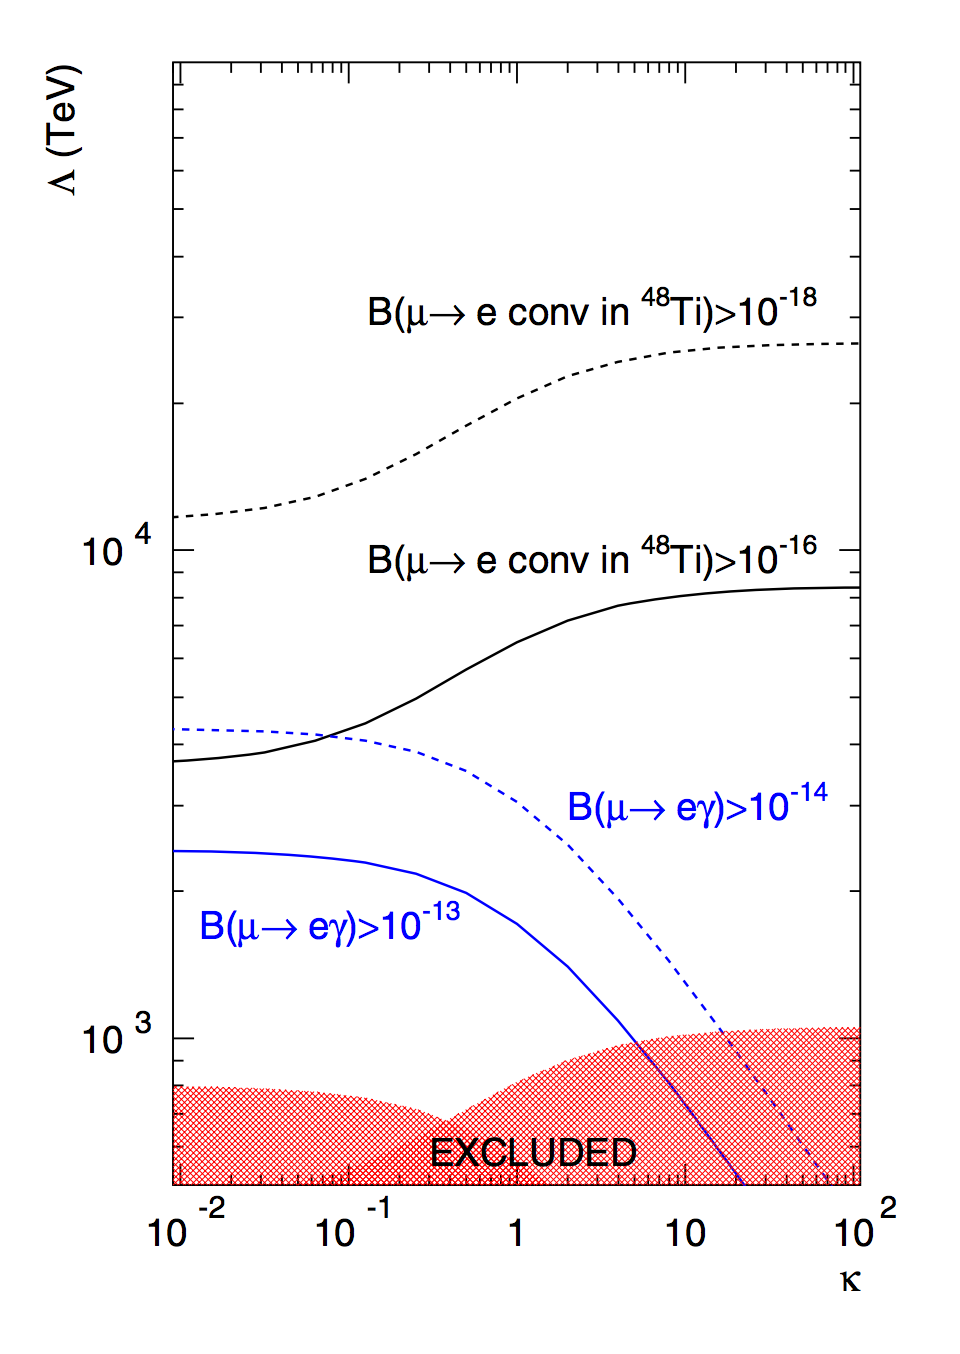
\includegraphics[width=\textwidth]{images/clfv_type1.png}
      \caption{\( \mu\rightarrow e \) in Ti and \( \mu\rightarrow e\gamma \) experiments}
    \end{subfigure}
    \begin{subfigure}[t]{0.49\textwidth}
      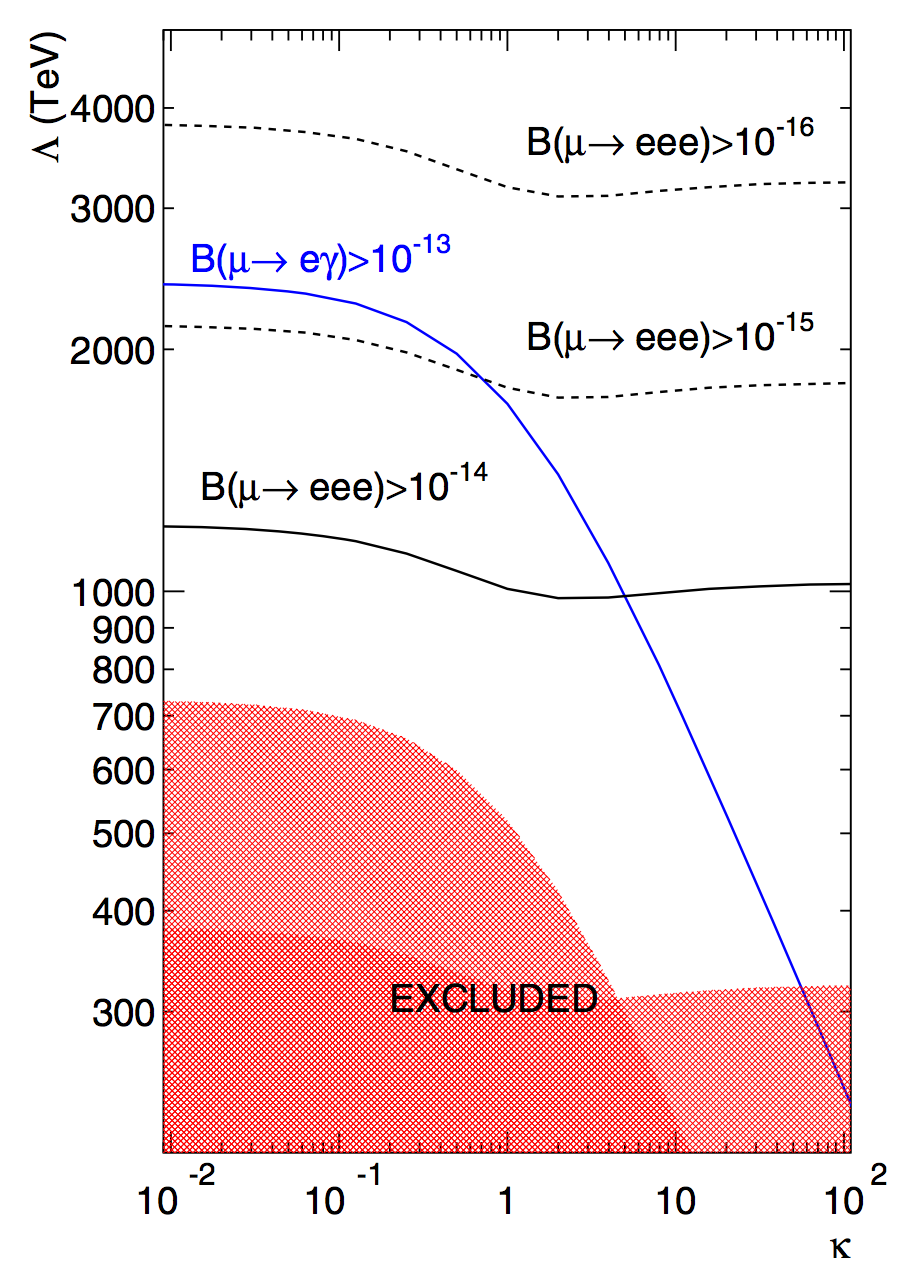
\includegraphics[width=\textwidth]{images/clfv_type2.png}
      \caption{\( \mu\rightarrow eee \) and \( \mu\rightarrow e\gamma \). The target sensitivity for \( \mu\rightarrow eee \) measurements at MuSIC is shown in the solid black line.}
    \end{subfigure}
    \caption{Effective mass scales, \(\Lambda\) for expected sensitivities to muon cLFV processes for various interaction strength ratios, \(\kappa\). Figures from \cite{effective_lagrangian_for_clfv}.}
  \label{fig:images_clfv_type2}
\end{figure}

% section charged_lepton_flavour_violation (end)
% chapter physics (end)
%%%%%%%%%%%%%%%%%%%%%%%%%%%%%%%%%%%%%%%%%%%%%%%%%%%
% part introduction (end)
%%%%%%%%%%%%%%%%%%%%%%%%%%%%%%%%%%%%%%%%%%%%%%%%%%%